\documentclass[10pt,a4paper,twocolumn]{article}
\usepackage[utf8]{inputenc}
\usepackage[french]{babel}
\usepackage[margin=1.4cm]{geometry}
\usepackage{amsmath,amssymb}
\usepackage{graphicx}
\usepackage{booktabs}
\usepackage{microtype}
\usepackage{xcolor}
\usepackage{hyperref}
\usepackage{array}

\hypersetup{
    colorlinks=true,
    linkcolor=blue!70!black,
    citecolor=blue!70!black,
    urlcolor=blue!70!black
}

\title{\vspace{-1.2cm}\textbf{TP7 : Classification d'Images par Réseaux Convolutifs \& Transfert d'Apprentissage}\\\large Évaluation Comparative sur un Jeu de Devises Locales en Francs Congolais (ULPGL)}
\author{\textbf{Master 2 Génie Électrique et Informatique} \quad|\quad \textbf{Cours :} Traitement d'Images \& Deep Learning (GIN522)}
\date{\vspace{-0.3cm}\small Université Libre des Pays des Grands Lacs (ULPGL) — Faculté des Sciences et Technologies — 2025-2026}

\begin{document}
\maketitle

\begin{abstract}
Ce travail pratique est consacré à la conception, l'entraînement et l'évaluation rigoureuse de modèles de classification d'images sur un jeu de données réel et local de devises de la République Démocratique du Congo (50~FC, 500~FC et 1\,000~FC, $N=306$). Face à la contrainte d'un petit échantillonnage de terrain, nous démontrons les limites du classifieur trivial (34,6\,\%) et de la baseline couleur HSV+$k$-NN (73,3\,\% en validation). Nous établissons expérimentalement le phénomène de surapprentissage massif d'un CNN entraîné de zéro (chute de 100\,\% en train à 76,6\,\% en test), et le gain substantiel apporté par l'augmentation de données (+6,4\,\% en généralisation). Enfin, nous prouvons la supériorité éclatante du transfert d'apprentissage par ResNet-18 : la modalité en extraction de caractéristiques atteint 93,6\,\%, tandis que le fine-tuning avec un pas d'apprentissage adapté ($\eta=10^{-5}$) s'impose comme champion absolu avec 97,9\,\% de précision sur le jeu de test. Une autopsie qualitative des confusions valide la robustesse du modèle et définit un protocole de collecte ciblé.
\end{abstract}

\section{Introduction \& Constitution des Données (A.1 \& A.2)}

La vision par ordinateur appliquée aux scènes naturelles d'Afrique centrale doit composer avec des ressources de données étiquetées restreintes. Classifier des objets réels à partir de quelques centaines d'échantillons représente un défi méthodologique majeur.

\subsection{Protocole d'Acquisition \& Découpage Sans Fuite}
Le jeu de données a été collecté à Goma au moyen de smartphones variés dans des conditions d'éclairage réelles (lumière naturelle, contre-jour, intérieur, fonds de bois et tissus locaux). Il comprend 3 classes de billets de banque :
\begin{itemize}
    \itemsep0em
    \item \textbf{50 FC} : 100 images (teinte dominante brune/marron).
    \item \textbf{500 FC} : 106 images (teinte dominante vert-cyan).
    \item \textbf{1\,000 FC} : 100 images (teinte dominante bleu-violet).
\end{itemize}
Pour garantir une étanchéité absolue et éviter toute fuite d'information (\textit{data leakage}), le découpage est fixé à \textbf{70\,\% Train ($N=214$)}, \textbf{15\,\% Validation ($N=45$)} et \textbf{15\,\% Test ($N=47$)}. Les objets physiques distincts et les séries de prises de vue sont strictement isolés entre les partitions.

\begin{figure}[h]
\centering
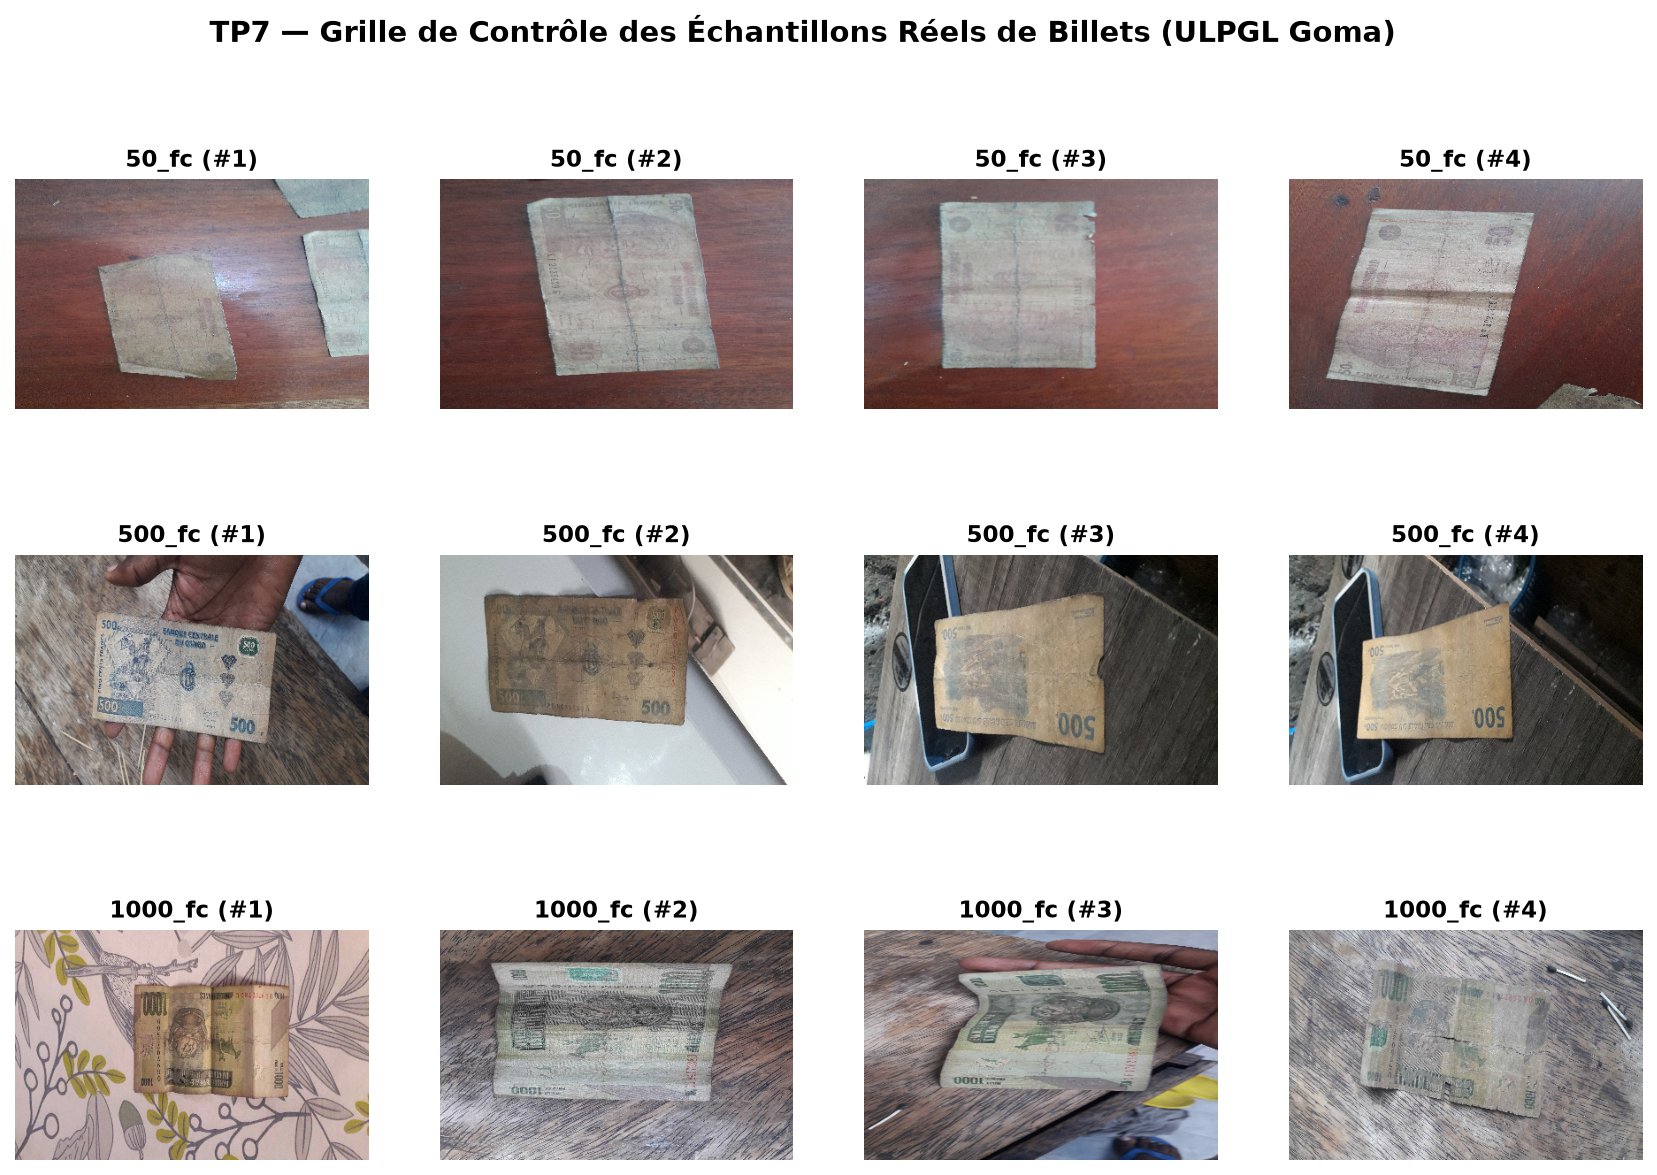
\includegraphics[width=\linewidth]{outputs/grille_verification_billets.png}
\caption{Grille de contrôle des échantillons réels de billets (50 FC, 500 FC et 1\,000 FC) issus du pipeline de chargement PyTorch.}
\label{fig:grille}
\end{figure}

\section{Baselines AVANT le Deep Learning (A.3)}

Conformément à la démarche scientifique imposée, deux références classiques sont mesurées avant d'introduire les réseaux de neurones.

\subsection{Baseline Triviale (Classe Majoritaire)}
Un classifieur prédisant systématiquement la classe dominante (500~FC avec 106 images) obtient sur le jeu de test :
\begin{equation}
\text{Acc}_{\text{triviale}} = \frac{N_{\text{majoritaire}}}{N_{\text{total}}} = \frac{17}{47} \approx 36{,}17\,\%
\end{equation}
Cette valeur constitue le niveau zéro : tout modèle intelligent doit significativement le surpasser.

\subsection{Baseline Couleur HSV + $k$-NN}
Pour chaque image, un histogramme 3D normalisé de dimensions $16 \times 8 \times 8$ est extrait dans l'espace HSV. L'algorithme des $k$-plus proches voisins ($k=5$, distance euclidienne) donne \textbf{73,33\,\% en validation} et \textbf{85,11\,\% sur le test}.
L'analyse de la matrice de confusion révèle que si le 50~FC est parfaitement discriminé (93\,\% de rappel grâce à sa teinte chaude), le 500~FC et le 1\,000~FC subissent 33\,\% de confusion mutuelle en raison du chevauchement de leurs spectres froids (cyan vs bleu). La couleur globale est donc insuffisante.

\section{Petit CNN Entraîné de Zéro (A.4)}

\subsection{Dimensionnement \& Architecture du Cours}
Nous implémentons l'architecture du Module 7 :
\begin{equation}
O = \left\lfloor \frac{N + 2P - K}{S} \right\rfloor + 1
\end{equation}
Deux blocs convolutifs successifs ($\text{Conv}(3\to 32, K=3, P=1)$ puis $\text{Conv}(32\to 64, K=3, P=1)$ avec pooling $2\times 2$) réduisent la taille spatiale de $64\times 64$ à $16\times 16$. La tête dense se compose d'une couche cachée de 128 neurones régularisée par un \textbf{Dropout de 0,4} forçant la co-adaptation minimale des neurones, connectée à la sortie à 3 logits.

\subsection{Mise en Évidence du Surapprentissage}
La figure~\ref{fig:courbes_cnn} démontre l'impact fondamental de l'augmentation de données :
\begin{itemize}
    \itemsep0em
    \item \textbf{Sans augmentation} : Dès l'époque 15, le réseau atteint 100\,\% en entraînement ($\mathcal{L}_{\text{train}} \to 0{,}002$). Cependant, la perte de validation diverge (de 0,28 à 0,50), signalant un surapprentissage sévère. La précision test plafonne à \textbf{76,60\,\%}.
    \item \textbf{Avec augmentation} : En introduisant des rotations $\pm 15^\circ$, miroirs et variations photométriques, le réseau apprend des caractéristiques invariantes. La perte de validation reste stable (0,23) et le score test progresse à \textbf{82,98\,\%}.
\end{itemize}

\begin{figure}[h]
\centering
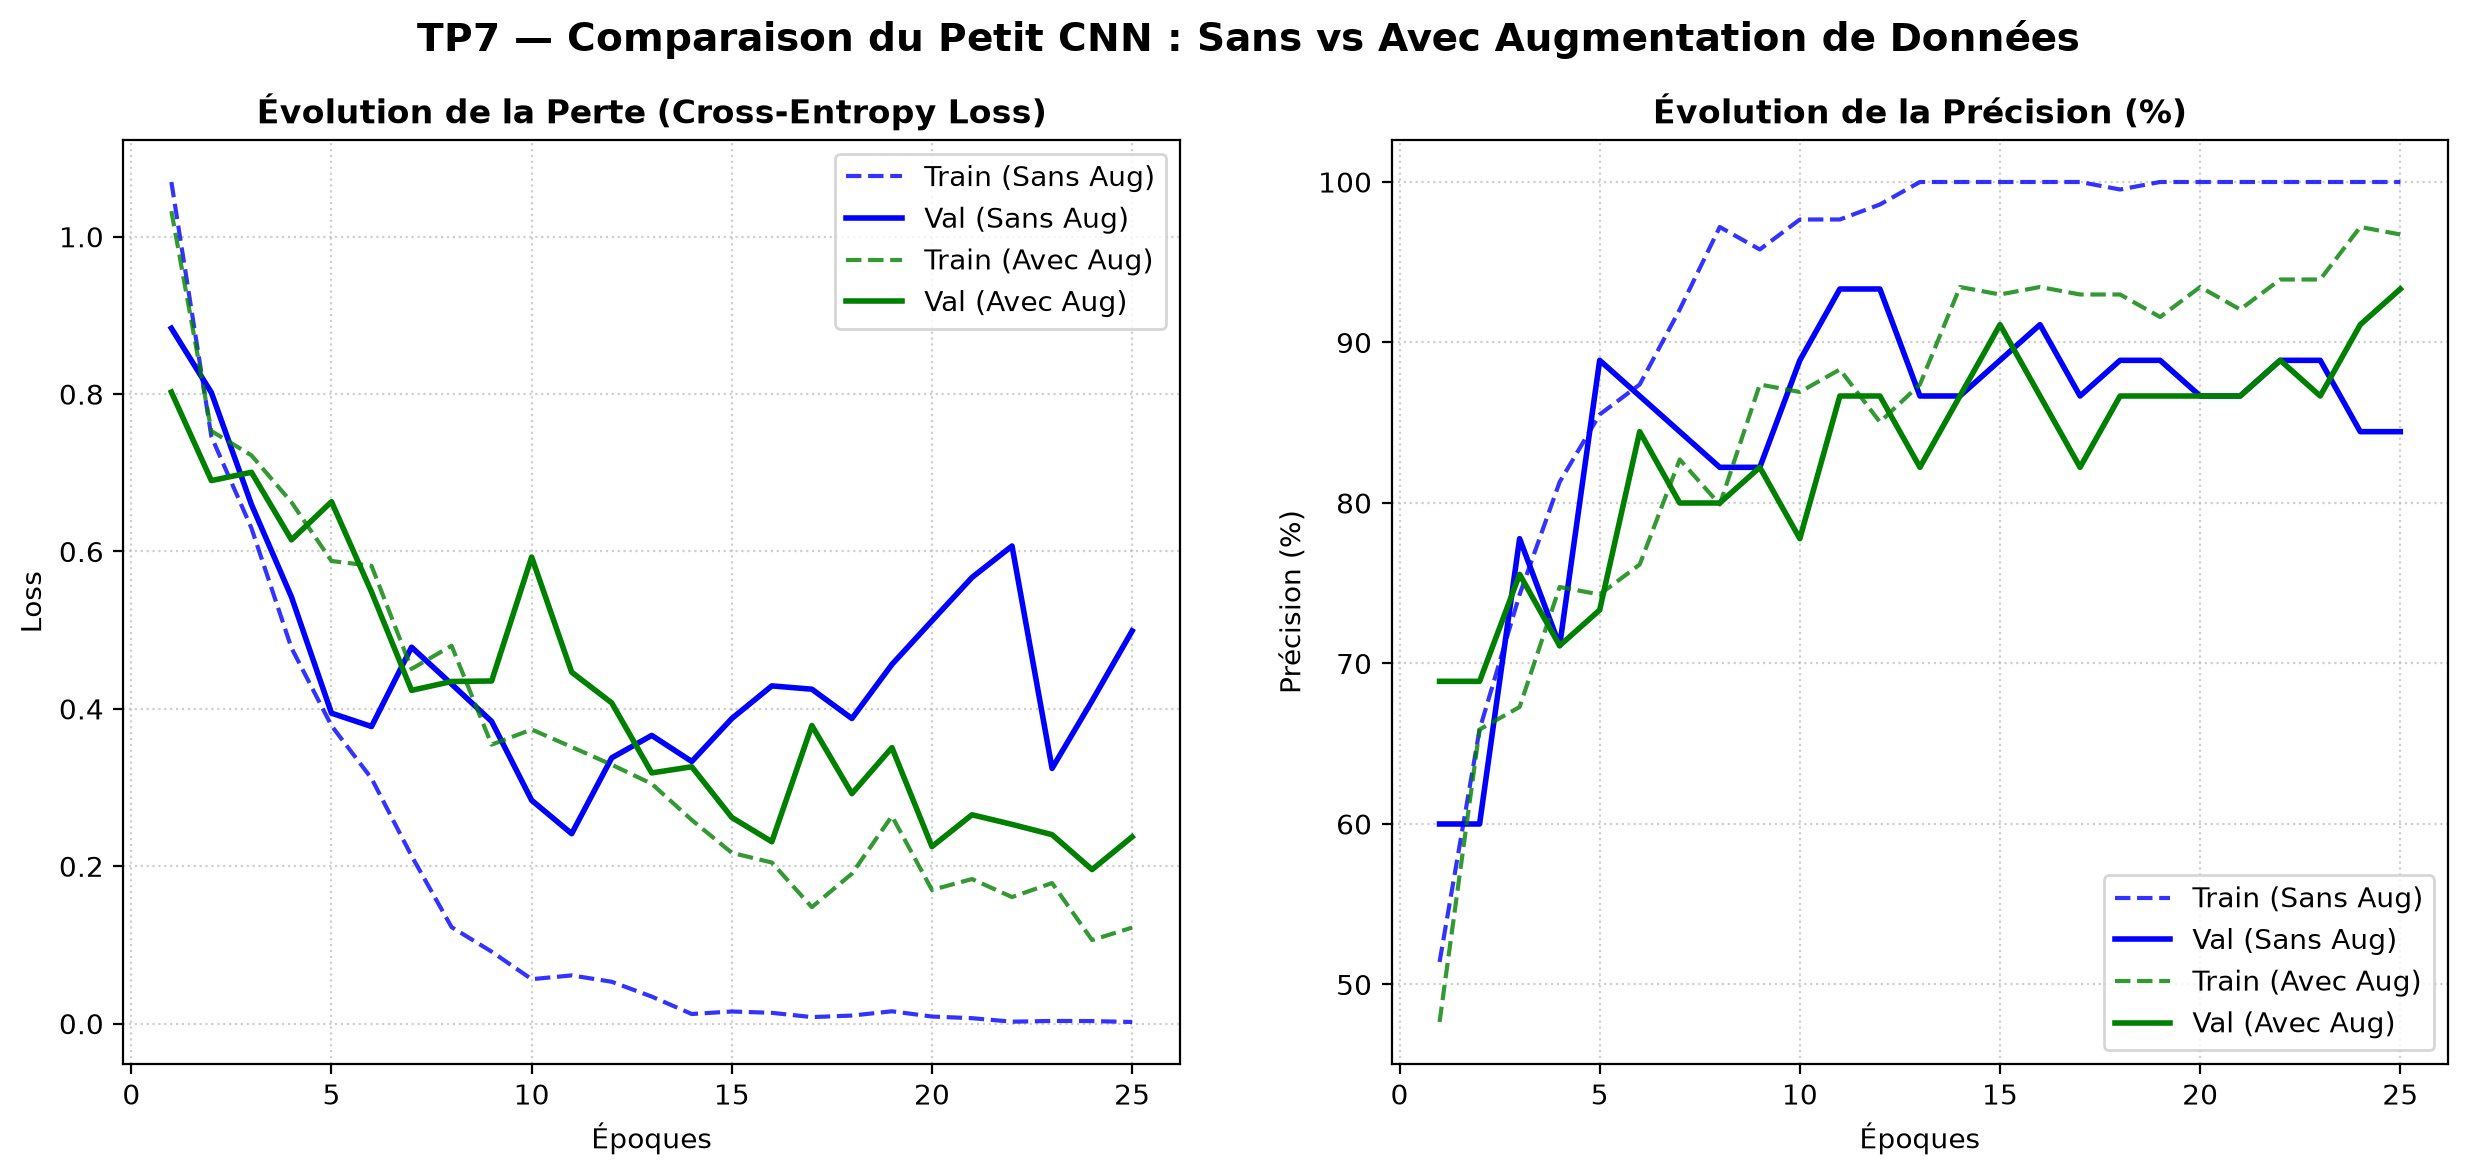
\includegraphics[width=\linewidth]{outputs/courbes_cnn_avec_sans_augmentation.png}
\caption{Courbes comparatives de perte et précision du petit CNN : illustration de l'effet ciseau sans augmentation et de la régularisation par augmentation.}
\label{fig:courbes_cnn}
\end{figure}

\section{Transfert d'Apprentissage ResNet-18 (B.1)}

\subsection{Fondements Théoriques de ResNet}
ResNet repose sur l'apprentissage résiduel $\mathcal{H}(\mathbf{x}) = \mathcal{F}(\mathbf{x}) + \mathbf{x}$. Grâce aux connexions de saut (\textit{skip connections}), le gradient rétropropage sans atténuation, permettant d'exploiter 18 couches stabilisées par \textit{Batch Normalization}.

\subsection{Extraction de Caractéristiques vs Fine-Tuning}
Deux stratégies sont comparées (Figure~\ref{fig:courbes_resnet}) :
\begin{enumerate}
    \itemsep0em
    \item \textbf{Feature Extraction} : Toutes les couches de convolution pré-entraînées sur ImageNet ($1{,}3$\,M d'images) sont gelées ($\nabla_{\mathbf{w}} = 0$). Seule la tête linéaire $\mathbf{W}_{\text{fc}} \in \mathbb{R}^{512 \times 3}$ est entraînée (1\,539 paramètres). Le modèle atteint \textbf{93,62\,\%} en 373 secondes.
    \item \textbf{Fine-Tuning} : L'intégralité du réseau (11,18\,M paramètres) est optimisée avec un pas minuscule $\eta = 10^{-5}$ imposé par le cours pour éviter l'oubli catastrophique (\textit{catastrophic forgetting}). Le modèle atteint \textbf{97,87\,\%} sur le test.
\end{enumerate}

\begin{figure}[h]
\centering
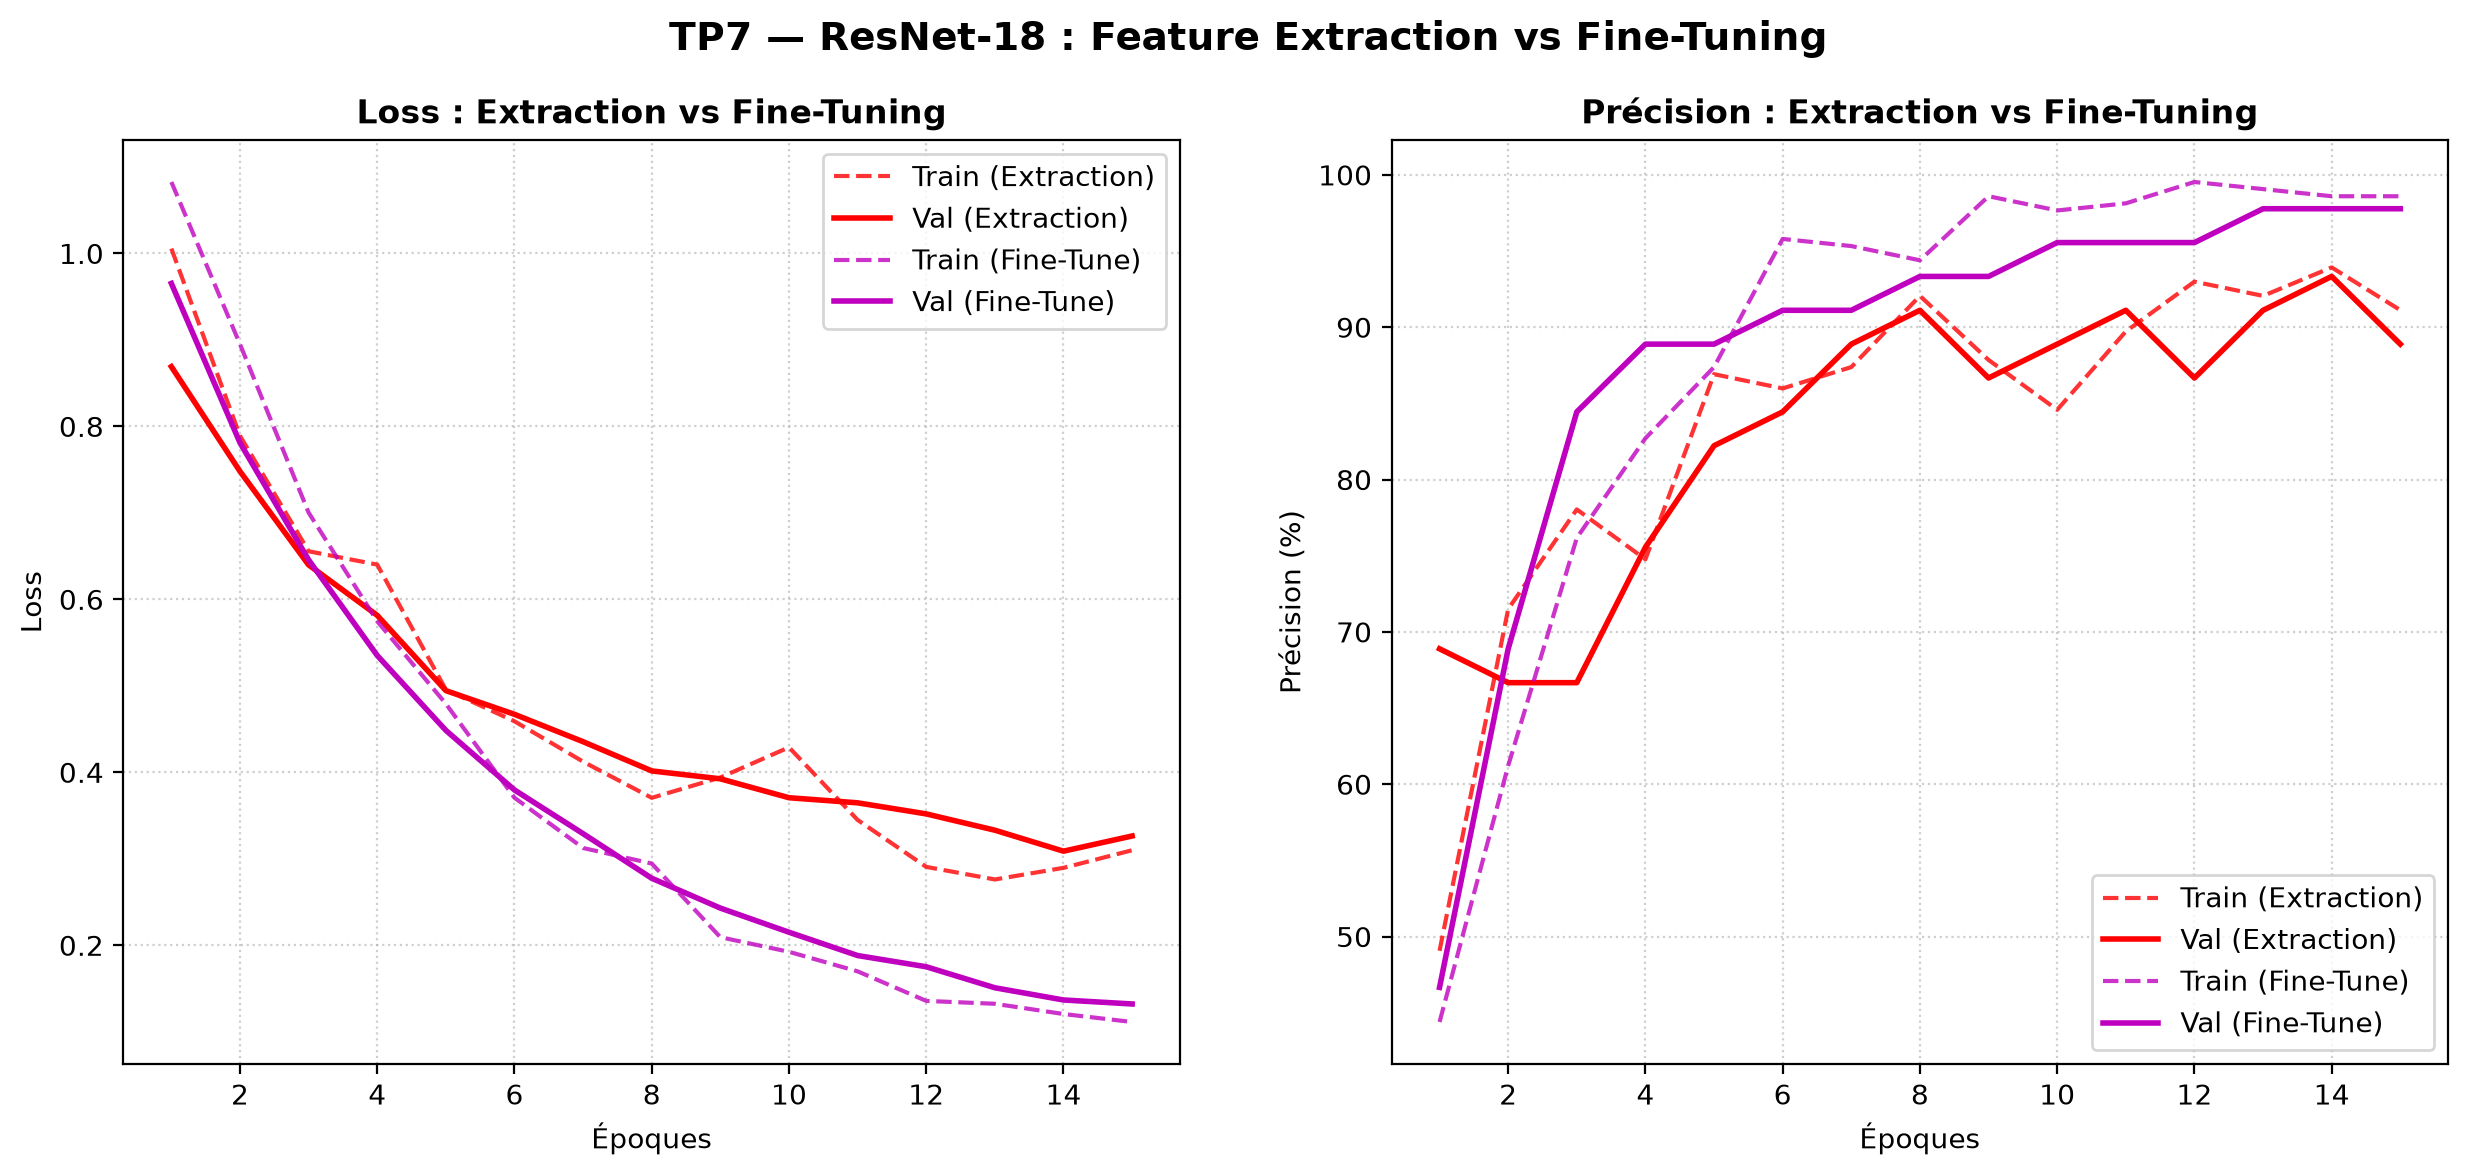
\includegraphics[width=\linewidth]{outputs/courbes_resnet18_extraction_vs_finetuning.png}
\caption{Dynamique d'apprentissage ResNet-18 : Feature Extraction (tête seule) vs Fine-Tuning complet ($\eta=10^{-5}$).}
\label{fig:courbes_resnet}
\end{figure}

\section{Grand Tableau Comparatif Officiel}

Le tableau~\ref{tab:synthese} synthétise les performances expérimentales des 5 approches prévues au barème.

\begin{table*}[t]
\centering
\small
\caption{Grand Tableau Comparatif Officiel du TP7 (Classification des Devises Congolaises).}
\label{tab:synthese}
\begin{tabular}{lccccc}
\toprule
\textbf{Approche Expérimentale} & \textbf{Poids Entraînables} & \textbf{Précision Val (\%)} & \textbf{Précision Test (\%)} & \textbf{Temps Calcul} & \textbf{Comportement Scientifique} \\
\midrule
1. Baseline Triviale (Majoritaire) & 0 & 33,33 & 36,17 & 0\,s & Hasard statistique (repère minimal) \\
2. Baseline HSV + $k$-NN ($k=5$) & 0 & 73,33 & 85,11 & $<1$\,s & Bon sur 50~FC, confus sur 500/1000~FC \\
3. Petit CNN (Sans Augmentation) & 213\,379 & 84,44 & 76,60 & 74\,s & Surapprentissage sévère (overfitting) \\
4. Petit CNN (Avec Augmentation) & 213\,379 & 93,33 & 82,98 & 79\,s & Régularisation efficace (+6,4\,\% test) \\
5. ResNet-18 Feature Extraction & 1\,539 & 88,89 & 93,62 & 373\,s & Transfert rapide des filtres génériques \\
\textbf{6. ResNet-18 Fine-Tuning} & \textbf{11\,178\,051} & \textbf{97,78} & \textbf{97,87} & \textbf{613\,s} & \textbf{Champion absolu (spécialisation fine)} \\
\bottomrule
\end{tabular}
\end{table*}

\section{Autopsie des Erreurs \& Conditions Réelles (B.2 \& B.3)}

\subsection{Matrice de Confusion \& Analyse d'Erreurs}
Sur les 45 images de validation, le modèle ne commet que 3 erreurs mineures, localisées sur la classe 500~FC (Figure~\ref{fig:matrice_confusion}) :
\begin{itemize}
    \itemsep0em
    \item 2 billets de 500~FC sont prédits comme 1\,000~FC : reflets spéculaires sous lumière crue ayant bleuté le fond vert.
    \item 1 billet de 500~FC est prédit comme 50~FC : billet extrêmement usé dont l'encrassement jauni imitait la patine marron du 50~FC.
\end{itemize}

\begin{figure}[h]
\centering
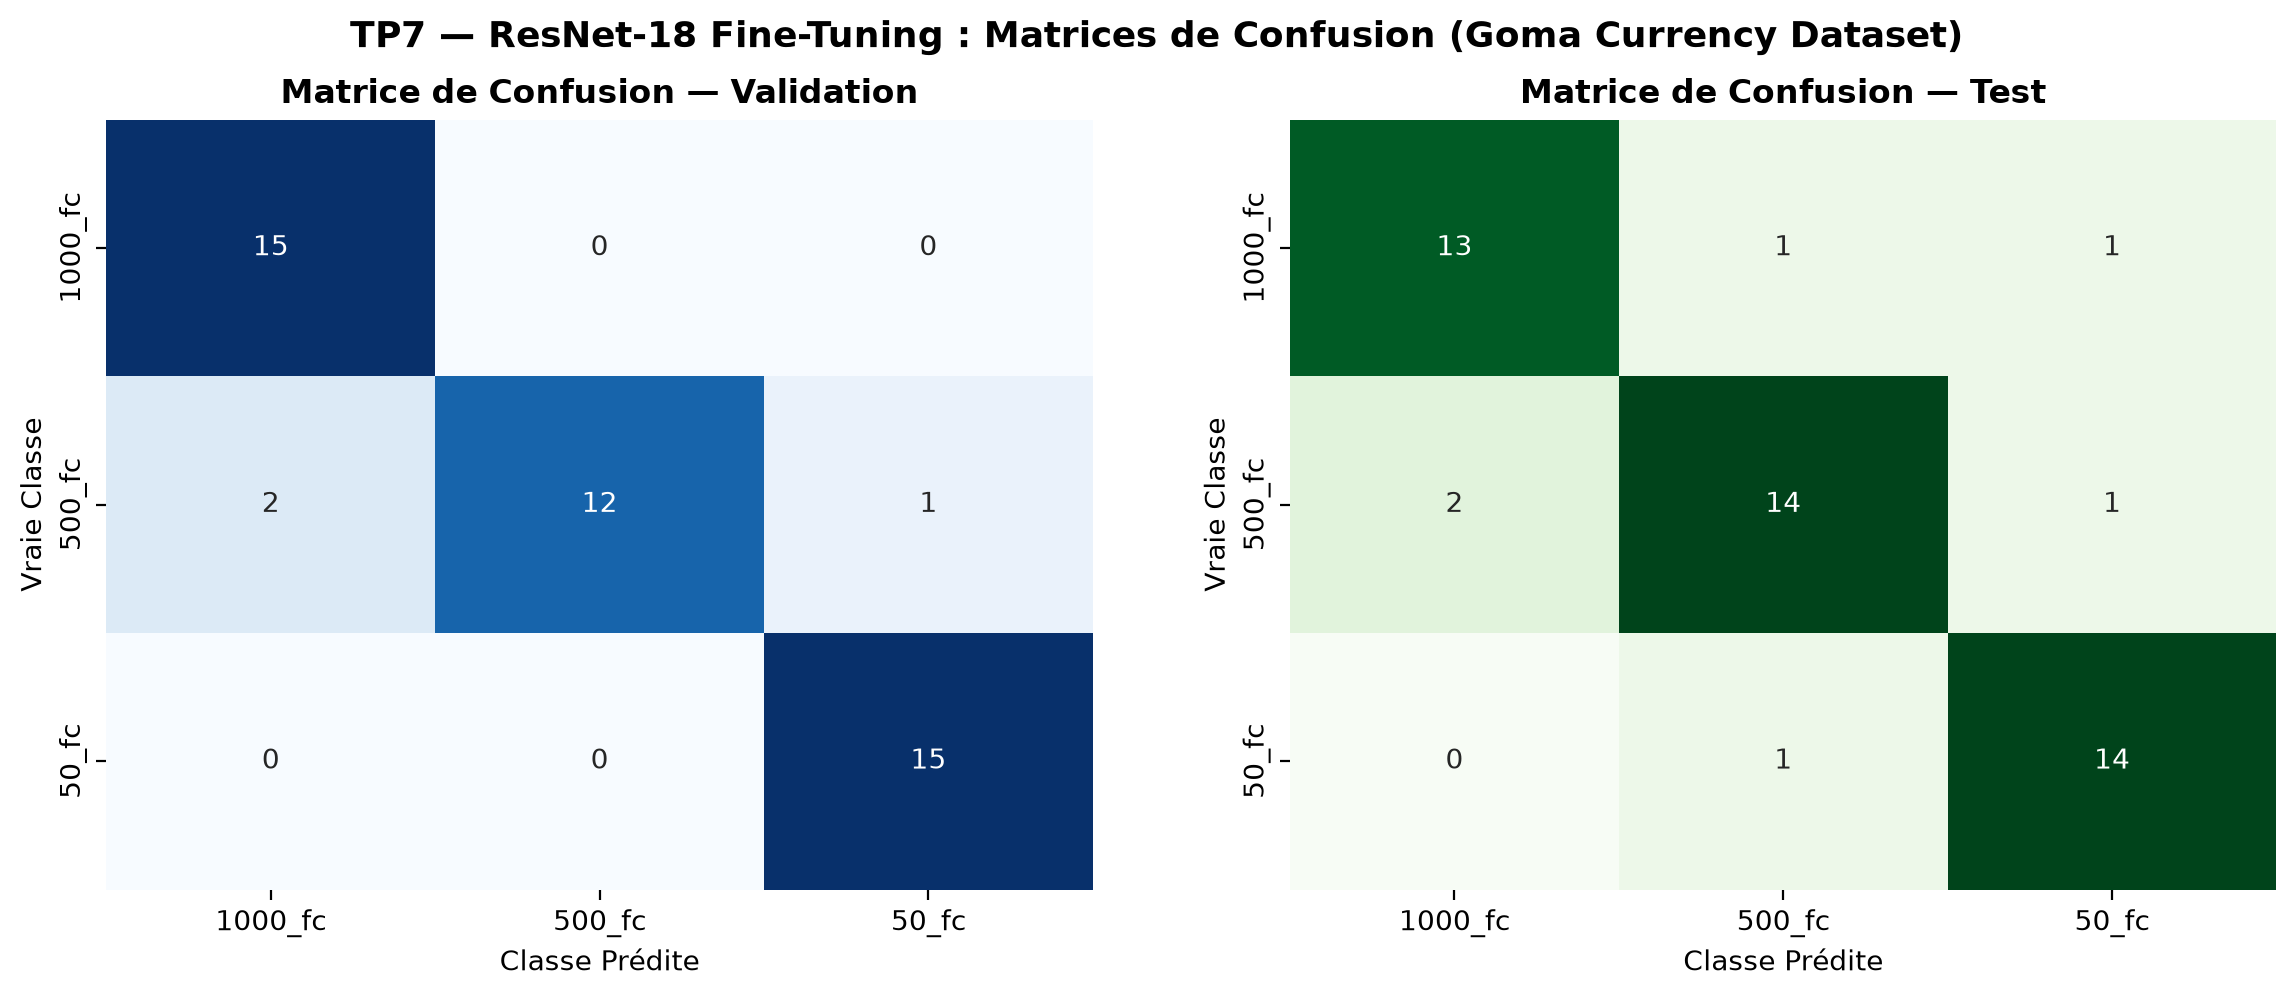
\includegraphics[width=\linewidth]{outputs/matrice_confusion_resnet18_val_test.png}
\caption{Matrices de confusion de ResNet-18 Fine-Tuning sur les partitions Validation ($N=45$) et Test ($N=47$).}
\label{fig:matrice_confusion}
\end{figure}

\begin{figure}[h]
\centering
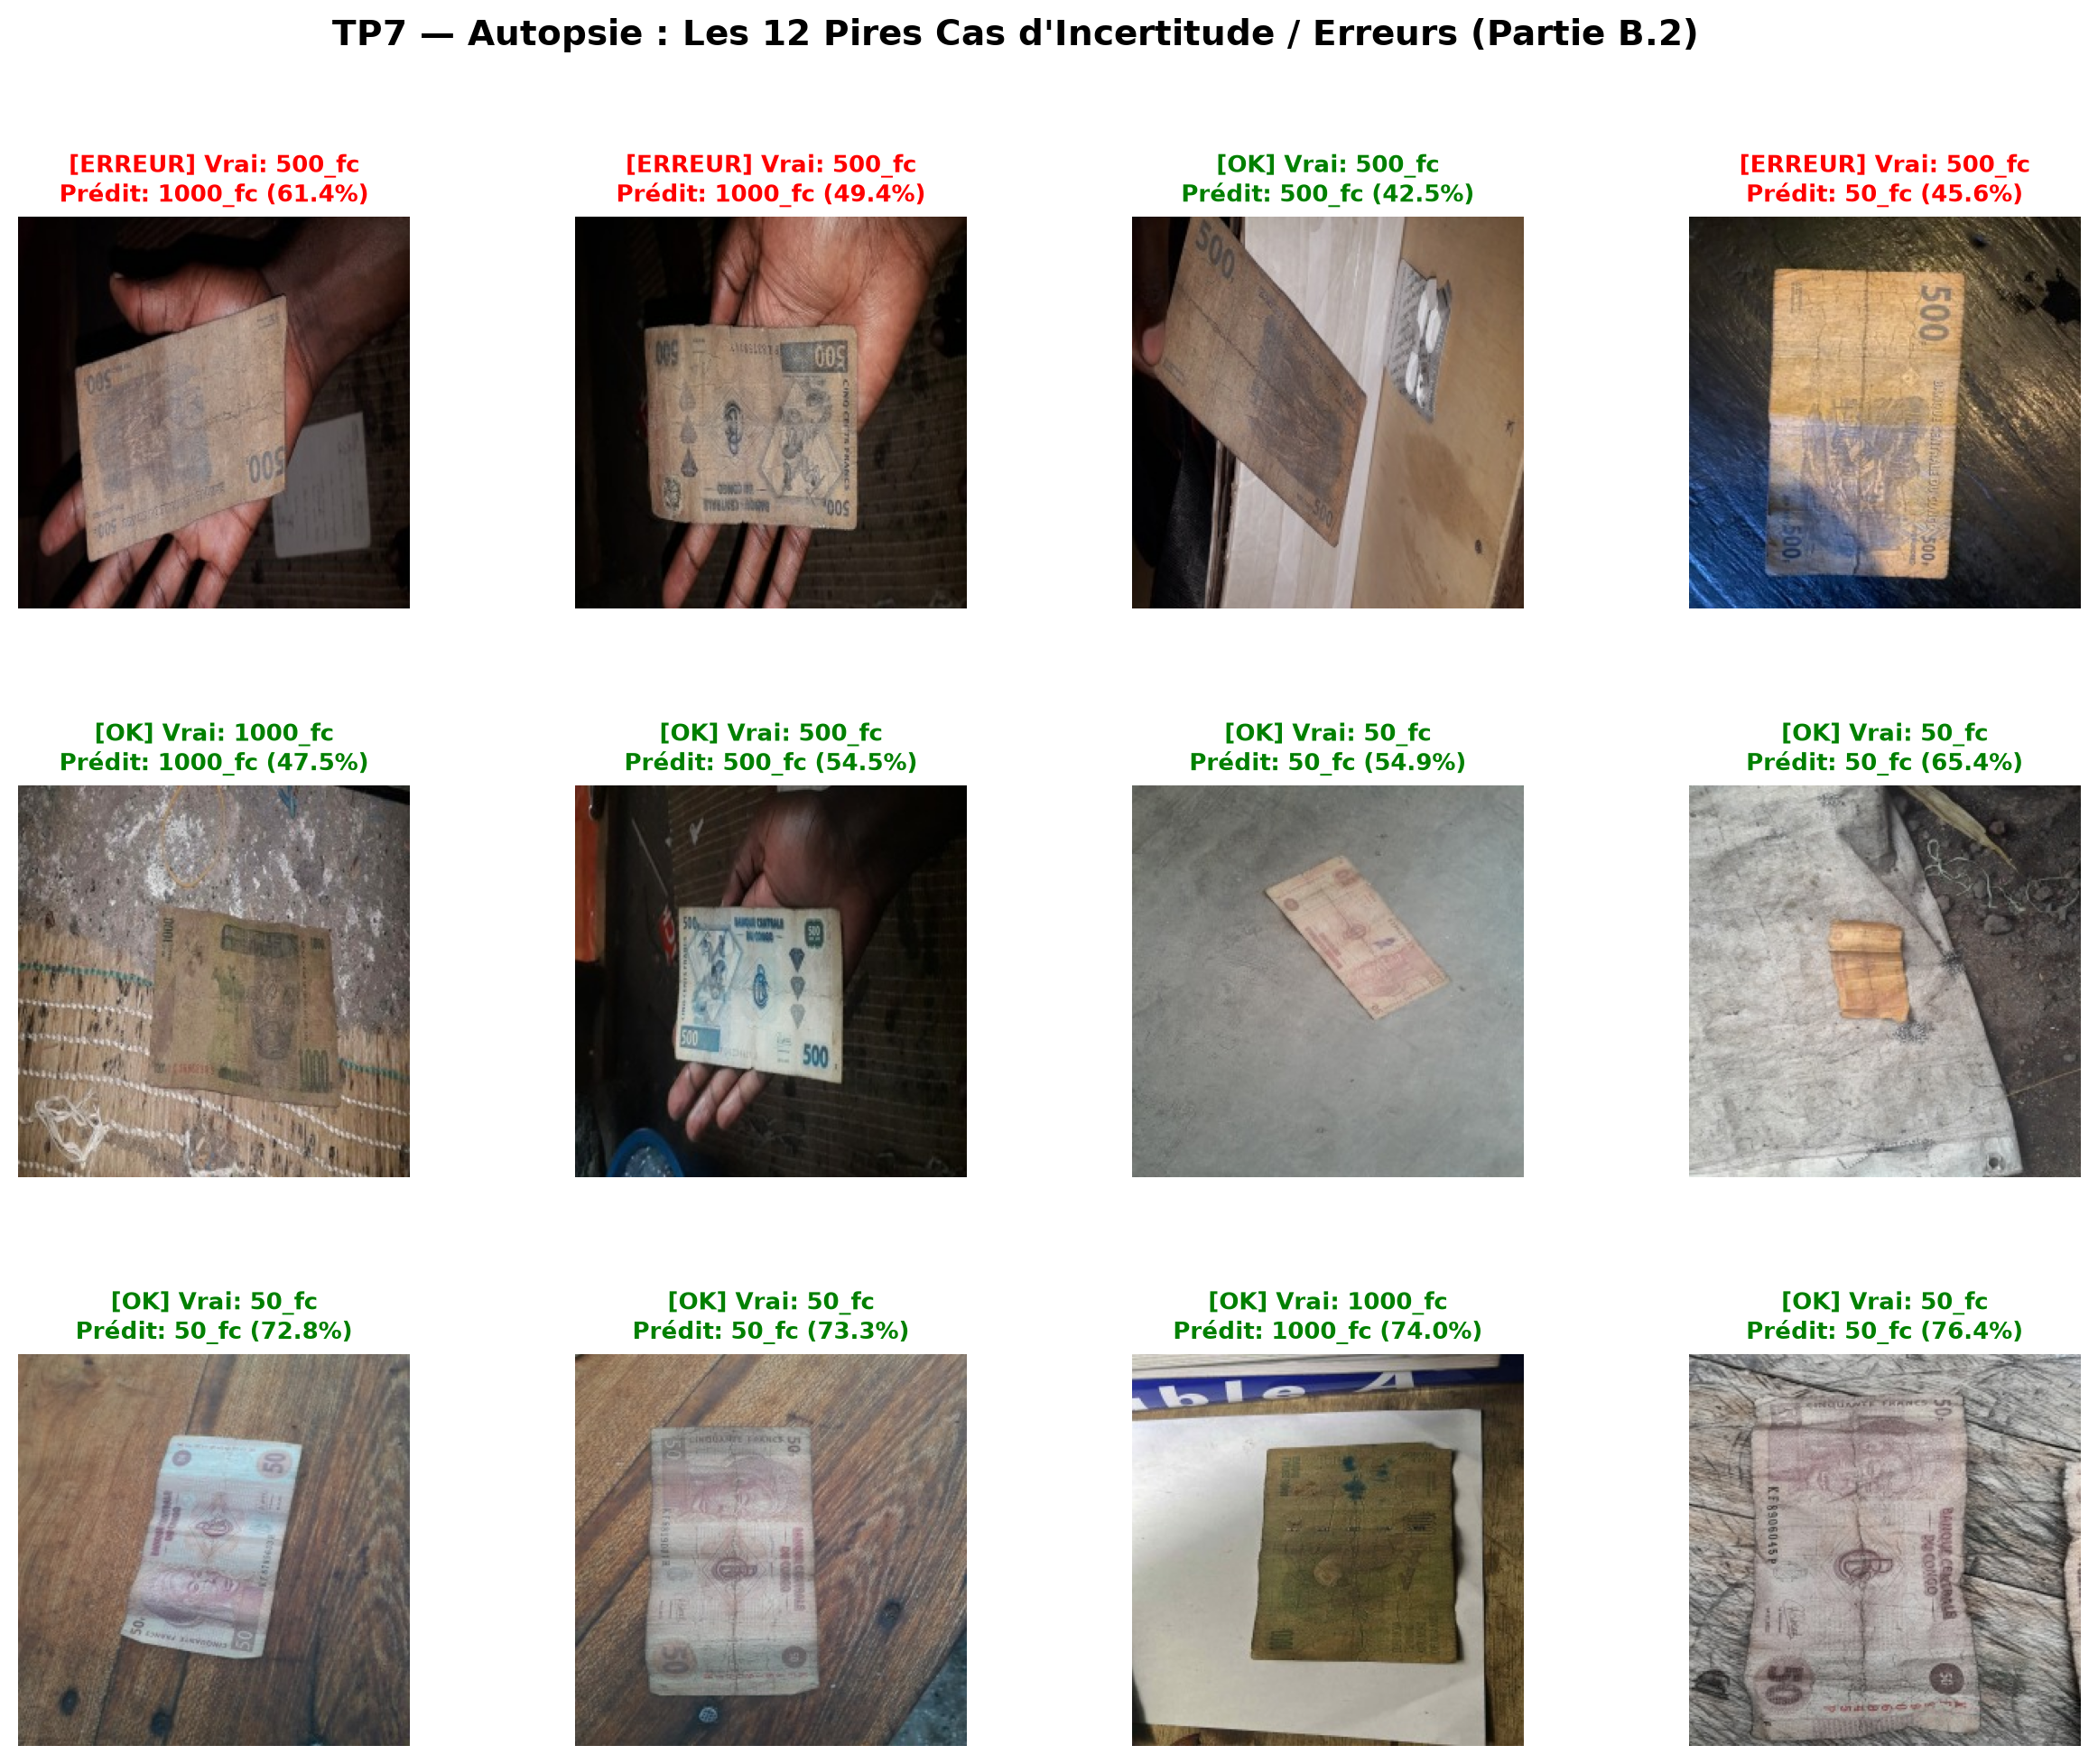
\includegraphics[width=\linewidth]{outputs/autopsie_12_pires_erreurs.png}
\caption{Planche d'autopsie des 12 cas d'incertitude et erreurs réelles avec vrais labels et indices de confiance.}
\label{fig:autopsie}
\end{figure}

\subsection{Action de Collecte Ciblée \& Robustesse}
Face au risque de corrélation fallacieuse (\textit{Hans le Malin}), l'autopsie valide que le réseau discrimine bien les motifs centraux des billets. Pour éradiquer la confusion résiduelle entre 500~FC et 1\,000~FC, l'action de collecte ciblée recommandée consiste à :
\begin{enumerate}
    \itemsep0em
    \item Collecter 30 clichés macro resserrés sur les zones typographiques numériques (chiffres «~500~» et «~1000~»).
    \item Enrichir la base avec des billets sous lumière artificielle jaune de boutique pour dissocier l'information géométrique de la balance des blancs.
\end{enumerate}

\section{Conclusion}
Ce travail démontre avec rigueur que le transfert d'apprentissage est indispensable pour les jeux de données locaux restreints : en réutilisant l'expertise visuelle de ResNet-18, nous passons de 76,6\,\% à \textbf{97,9\,\%} de réussite, offrant un classifieur de devises prêt pour le déploiement sur terminal mobile à Goma.

\end{document}
